\chapter{Zielspezifikation ( 5 \%)}



% Wie das letzte kap gezeig hat ..
% in diesem kap sollen zie ziele quali/quantifiziert werden


% tests in sektionen mit angeben


% funktional, tests, szstemanforderunge? bessereer name
% abgrenzungen
% zusammenfassung 
%   - im wesentlichen soll \ldots. prototypisch & exemplarisch
%   anhand .. soll ein loesungskonz vorgestellt werden

%Was soll konkret gelöst werden. Hierzu gehören u.a.
%    -    Anforderungskatalog
%    -    Use-Cases
%    -    Pflichtenheft
%    -    Testkriterien
%    -    ... 


\begin{verbatim}
- funktional + use-cases
- systemspez anforderungen
- testkriterien
-



% kann/soll kriterien
\section{anforderungen system}


\section{funktionen}
\section{Funktionenale Anforderungen}
% evtl incl use-cases
\begin{verbatim}


- ausfallsicherheit bei absturz/beendigung
  von systemkomponenten

- projekt verwalten
- annahme/generieren von aufrtraegen
  - matrix mit

- erstellung/management von arbeitspacketen
  - von matrix
- abarbeitung von arbeitspacketen
  - scm
  - prozesse
- analyse von
  - zeitserien ueber projekte
  - auftraegen
  - arbeitspackete

  - ext analyse sommer projekt
  - ext regressionsanalyse (theorie) ?
\end{verbatim}

\section{Use Cases}



\begin{figure}[ht]
  \label{fig:use-case-muss}
  \begin{center}
      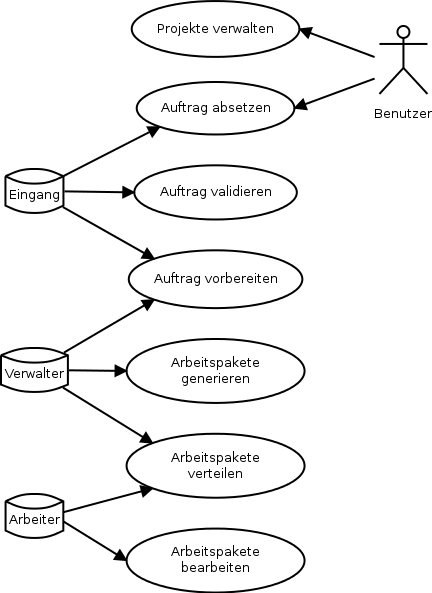
\includegraphics[width=0.7\textwidth]{imageinput/use-case-muss.png}
  \end{center}
  \caption{\"Ubersicht Use Cases - Muss}
\end{figure}


\begin{verbatim}
- build achsen ??

- extensions
  - regressionstest
  - testanalyse

- alte usecases
  - junitxml beispiel
  - stdout beispiel

- neue use-cases
  - workdir diff/tarball
  - auswertung zeitserien <addon>
  - datenanalyse beispiel sommer <addon>
\end{verbatim}


\section{rahmenbed}

\subsection{konkr}?
- testen notwendig
- das system selber ci unterziehen

\subsection{feststellung}
 - regeln


-----

\subsection{Unit tests ?}


\begin{verbatim}
- verweis auf grobentwurf?
- hilfskomponenten
- eregeben sich bei impl
\end{verbatim}

\subsection{funktionale Tests}

\begin{verbatim}
- einzelnen komponenten
  - auftragseingang
  - aftragsvorbereitung
  - auftragsabarbeitung
  - schritte durchlaufen

- schrittypen durchfuehren
 - prozess
 - python ?
 - scm


\end{verbatim}

\subsection{systemtests}

\begin{verbatim}
- komponentendurchlauf
- durchlauf komplettsystem
- resultate beispiel datenanalyse

\end{verbatim}

